\documentclass[tikz,border=10pt]{standalone}
\usepackage{amsmath}
\usepackage{amssymb}
\usepackage{tikz}
\usetikzlibrary{arrows.meta,calc}

\definecolor{figazul}{RGB}{2,132,199}
\definecolor{figrojo}{RGB}{220,38,38}
\definecolor{figverde}{RGB}{22,163,74}

\begin{document}
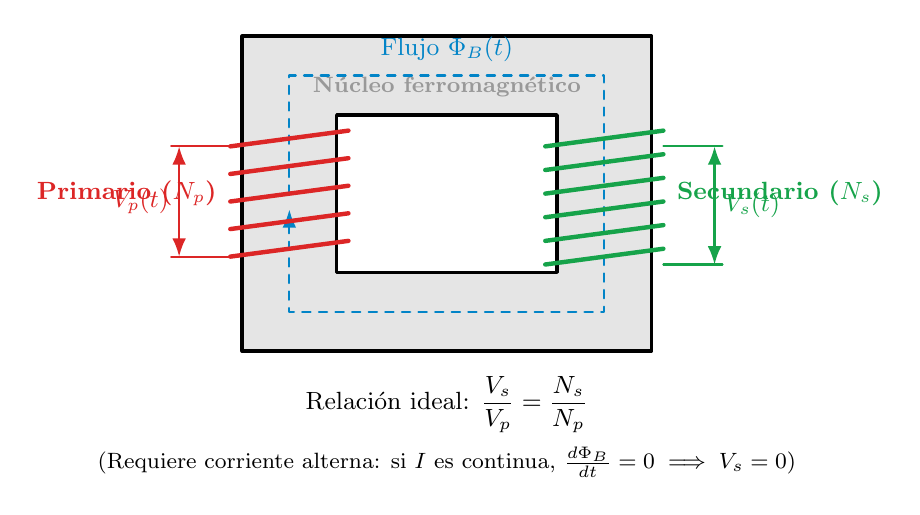
\begin{tikzpicture}[>=Latex, line cap=round, line join=round]
  % Núcleo ferromagnético cerrado (rectángulo exterior e interior)
  % Exterior: de x = -2.6 a 2.6, de y = -2.0 a 2.0
  % Interior: de x = -1.4 a 1.4, de y = -1.0 a 1.0
  \draw[very thick, fill=gray!20, even odd rule]
    (-2.6, -2.0) rectangle (2.6, 2.0)
    (-1.4, -1.0) rectangle (1.4, 1.0);
  \node[above, font=\footnotesize\bfseries, color=gray!80] at (0, 1.1) {N\'ucleo ferromagn\'etico};

  % Línea de flujo magnético circulating (Phi_B) en el interior del núcleo
  \draw[->, thick, dashed, color=figazul] (-2.0, 0) -- (-2.0, 1.5) -- (2.0, 1.5) -- (2.0, -1.5) -- (-2.0, -1.5) -- (-2.0, -0.2);
  \node[above, font=\small, color=figazul] at (0, 1.55) {Flujo $\Phi_B(t)$};

  % Devanado primario (columna izquierda): N_p vueltas
  \foreach \y in {-0.7, -0.35, 0.0, 0.35, 0.7} {
    \draw[ultra thick, color=figrojo] (-2.75, \y-0.1) -- (-1.25, \y+0.1);
  }
  % Terminales del primario
  \draw[thick, color=figrojo] (-2.75, 0.6) -- (-3.5, 0.6);
  \draw[thick, color=figrojo] (-2.75, -0.8) -- (-3.5, -0.8);
  \draw[<->, thick, color=figrojo] (-3.4, -0.8) -- (-3.4, 0.6) node[midway, left, color=figrojo, font=\small] {$V_p(t)$};
  \node[left, font=\small\bfseries, color=figrojo] at (-2.8, 0) {Primario ($N_p$)};

  % Devanado secundario (columna derecha): N_s vueltas
  \foreach \y in {-0.8, -0.5, -0.2, 0.1, 0.4, 0.7} {
    \draw[ultra thick, color=figverde] (1.25, \y-0.1) -- (2.75, \y+0.1);
  }
  % Terminales del secundario
  \draw[thick, color=figverde] (2.75, 0.6) -- (3.5, 0.6);
  \draw[thick, color=figverde] (2.75, -0.9) -- (3.5, -0.9);
  \draw[<->, thick, color=figverde] (3.4, -0.9) -- (3.4, 0.6) node[midway, right, color=figverde, font=\small] {$V_s(t)$};
  \node[right, font=\small\bfseries, color=figverde] at (2.8, 0) {Secundario ($N_s$)};

  % Ecuación fundamental del transformador ideal
  \node[below, font=\small, align=center] at (0, -2.2) {
    Relaci\'on ideal: $\displaystyle\frac{V_s}{V_p} = \frac{N_s}{N_p}$ \\[4pt]
    \footnotesize(Requiere corriente alterna: si $I$ es continua, $\frac{d\Phi_B}{dt} = 0 \implies V_s = 0$)
  };

\end{tikzpicture}
\end{document}
